%&latex
% !TeX program = lualatex
% Use A4 explicitly so output is consistent across systems.
\documentclass[a4paper,12pt]{article}

% Page layout.
\usepackage[margin=1in]{geometry}
\setlength{\parindent}{0pt}
\setlength{\parskip}{0.6em}

% Fonts.
\usepackage{fontspec}
\setmainfont{TeX Gyre Termes}
\setmonofont{Noto Sans Mono}
\newfontfamily{\treefont}{Noto Sans Mono}

% Syntax-highlighted code blocks.
% Compile with shell escape enabled when using minted.
\usepackage{xcolor}
\usepackage{minted}
\setminted{
  fontsize=\small,
  breaklines=true,
  autogobble=true,
  frame=single,
  framesep=2mm
}

% Clickable cross-references and links. Keep this near the end of the preamble.
\usepackage[colorlinks=true, linkcolor=blue, urlcolor=blue]{hyperref}
\usepackage{xurl}
\newcommand{\code}[1]{\texttt{\nolinkurl{#1}}}

% for images
\usepackage{graphicx}
\usepackage{float}

\title{Workshop Notes: Running an LLM Locally}
\author{Yang Shen}
\date{}

\begin{document}

\maketitle

\section{Overview}

This document shows how to run a small language model on your own computer. You will also use it with \textbf{Pi}, an agentic command-line tool.\footnote{If you have heard of OpenClaw, Pi is the lower-level tool that OpenClaw is built on.} The examples use \textbf{llama.cpp} to run the model, and \textbf{Qwen3-0.6B} as the practice model.

The goal is not to build the fastest or most powerful local AI system. The goal is to learn the general workflow: install the tools, download a model file, start a local model server, connect an application such as Pi to it, and try a few tasks. We use a small model so the workshop can work on most personal computers.

These notes are split into two main parts. The quick start gives the shortest path to a working local model. The later sections explain the tools, files, commands, and choices in more detail.

\section{Quick Start}

In this workshop, we will provide these files if you have not downloaded them yet:

\begin{itemize}
\item \texttt{Docker Desktop Installer.exe}
\item \texttt{Docker.amd64.dmg}
\item \texttt{Docker.arm64.dmg}
\item \texttt{llama.cpp.arm64.tar.gz}
\item \texttt{llama.cpp.tar.gz}
\item \texttt{pi-docker-image.arm64.tar.gz}
\item \texttt{pi-docker-image.tar.gz}
\item \verb|Qwen3-0.6B-UD-IQ1_S.gguf|
\item \verb|Qwen3-0.6B-UD-Q4_K_XL.gguf|
\item \texttt{Qwen3-0.6B-BF16.gguf}
\item \texttt{model.json}
\end{itemize}

The download links will be shared during the workshop.

\subsection{Install Docker}

You do not have to use Docker to run an LLM locally. In this workshop, we use Docker to make setup easier. A Docker image is like a ready-made box. It already contains the tools and settings we need. You do not need to install each part by hand.

Docker also keeps the workshop tools separate from the rest of your system. After the workshop, you can remove the images and containers easily. In a later section, we will introduce how to set up the runtime without Docker. We will also talk about why Docker can still be useful.

\subsubsection{Install Docker Desktop on Windows}

Official guide: \url{https://docs.docker.com/desktop/setup/install/windows-install/}

The general steps are:

\begin{enumerate}
\item Install WSL.\footnote{WSL stands for Windows Subsystem for Linux. It's a component available on Windows 10 and 11. It is a backend for Docker on Windows. It is outside the scope of this workshop so we are not going to talk the details of it.} First, check whether WSL is installed, open \textbf{PowerShell} or \textbf{Windows Command Prompt} and run this command:

\begin{minted}{bash}
wsl --version
\end{minted}

If you can see lines like "WSL version", then WSL is ready. Otherwise, open PowerShell or Windows Command Prompt \textbf{as an administrator} and run:

\begin{minted}{bash}
wsl --install
\end{minted}

This might take some time. After the installation, run \verb|wsl --version| again. If it shows the version information, you can proceed to the next step. If an error blocks you from installing WSL, please refer to PLACEHOLDER.

\item Double-click \texttt{Docker Desktop Installer.exe}. Keep the default configuration:

\begin{itemize}
\item \textbf{Per-user installation} selected
\item \textbf{Use WSL2 instead of Hyper-V} checked
\end{itemize}

\begin{figure}[htbp]
\centering
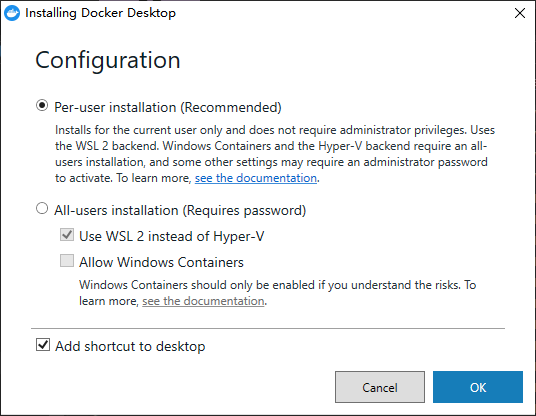
\includegraphics[width=0.8\textwidth]{assets/docker-windows-1.png}
\caption{Docker Desktop Installer for Windows}
\end{figure}

\item After the installation, open Docker Desktop. The first time you open it, click \textbf{Skip}, because sign-in is not required. If everything works, you should see the interface shown in Figure~\ref{fig:docker-windows-3}.

\begin{figure}[htbp]
\centering
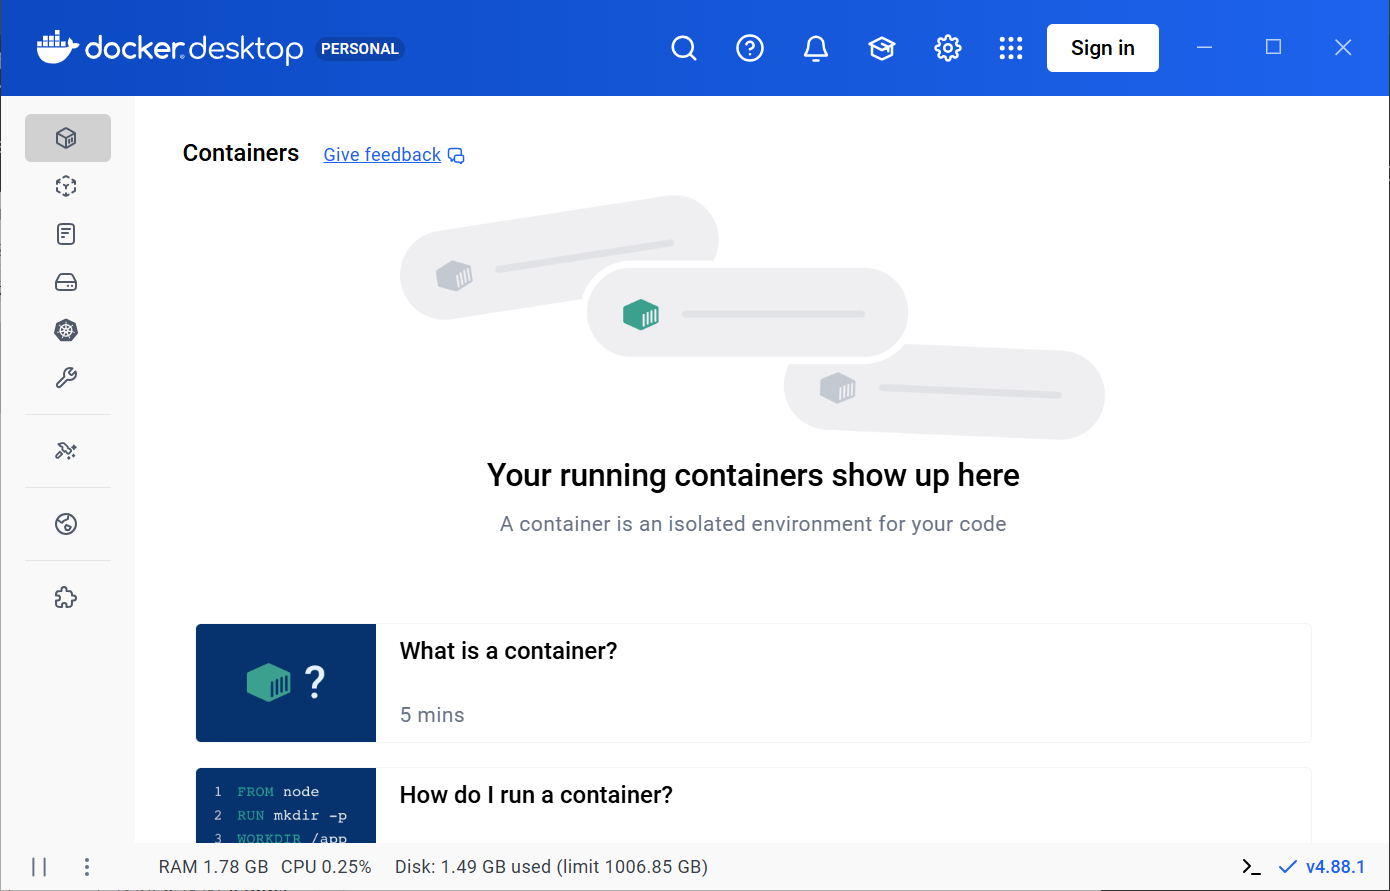
\includegraphics[width=0.8\textwidth]{assets/docker-windows-3.png}
\caption{Docker Desktop}
\label{fig:docker-windows-3}
\end{figure}
\end{enumerate}

\subsubsection{Install Docker Desktop on Mac}

Official guide: \url{https://docs.docker.com/desktop/setup/install/mac-install/}

Make sure your macOS version is at least \texttt{14.x}, and your Mac has at least 4 GB of RAM. Then choose the correct installer. If your Mac uses Apple silicon, such as an M1, M2, ..., M6 chip, choose \texttt{Docker Desktop for Mac With Apple silicon}. Otherwise choose \texttt{Docker Desktop for Mac with Intel chip}.

\begin{enumerate}
\item Double-click the downloaded \texttt{.dmg} file, then drag the icon to the \textbf{Applications} folder.
\item Double-click \texttt{Docker.app} in the \textbf{Applications} folder and start the installation.
\item Keep \textbf{Use recommended settings} selected.
\item Click \textbf{Skip}, because sign-in is not required.
\item Finally, you should see an interface similar to Figure~\ref{fig:docker-windows-3}.
\end{enumerate}

\subsubsection{Install Docker Engine on Linux}

Please follow the official guide for your Linux distribution: \url{https://docs.docker.com/engine/install/}

After installation, you may need to run Docker commands with \texttt{sudo}. If you want to run \texttt{docker} without \texttt{sudo}, follow the Linux post-installation guide: \url{https://docs.docker.com/engine/install/linux-postinstall/}

\subsection{Download and Import the Docker images}

If you use a Mac with Apple silicon, download \code{llama.cpp.arm64.tar.gz} and \code{pi-docker-image.arm64.tar.gz}. For other computers, download \code{llama.cpp.tar.gz} and \code{pi-docker-image.tar.gz}.

Then open a terminal. On Windows, you can use PowerShell or Windows Command Prompt. Run the commands for your computer:

\begin{minted}{bash}
# Mac with Apple silicon
docker load < llama.cpp.arm64.tar.gz
docker load < pi-docker-image.arm64.tar.gz

# other computers
docker load < llama.cpp.tar.gz
docker load < pi-docker-image.tar.gz
\end{minted}

After that, run \verb|docker image ls|. You should see these two images:

\begin{itemize}
\item \texttt{ghcr.io/ggml-org/llama.cpp:server}
\item \texttt{ghcr.io/codebar-shanghai/pi-docker-image:latest}
\end{itemize}

\subsection{Download the Language Model}

In this workshop, we use \textbf{Qwen3-0.6B}. We provide three model files:

\begin{itemize}
\item \texttt{Qwen3-0.6B-UD-Q4\_K\_XL.gguf}: use this one if possible. The commands in these notes use this file.
\item \texttt{Qwen3-0.6B-UD-IQ1\_S.gguf}: use this one if \texttt{Q4\_K\_XL} is still too large for your computer. You will need to update the model filename in the commands.
\item \texttt{Qwen3-0.6B-BF16.gguf}: try this one later if your computer has more free RAM. It keeps more precision, but it needs more memory. We will explain the names later.
\end{itemize}

\subsection{Run the Language Model}

The commands below are split into several lines to make them easier to read. The \texttt{\textbackslash} at the end of a line means the command continues on the next line. If you prefer, you can remove the \texttt{\textbackslash} characters and write each command as one long line.

If you are on \textbf{Windows}, and your files are under the folder \texttt{c:\textbackslash{}models}, run this command. If you used a different folder, replace \texttt{c:\textbackslash{}models} with your own folder.

\begin{minted}{bash}
docker run --rm -it \
  -p 8080:8080 \
  -v "c:\models:/models" \
  ghcr.io/ggml-org/llama.cpp:server \
  -m /models/Qwen3-0.6B-UD-Q4_K_XL.gguf \
  -c 32768 \
  --port 8080
\end{minted}

If you are on \textbf{Linux} or \textbf{macOS}, and your model files are in \texttt{\$HOME/models}\footnote{\textbf{\texttt{\$HOME}} means your home folder.}, run this command. If you used a different folder, replace \texttt{\$HOME/models} with your own folder.

\begin{minted}{bash}
docker run --rm -it \
  -p 8080:8080 \
  -v "$HOME/models:/models" \
  ghcr.io/ggml-org/llama.cpp:server \
  -m /models/Qwen3-0.6B-UD-Q4_K_XL.gguf \
  -c 32768 \
  --port 8080
\end{minted}

Here is a short explanation of the command. \texttt{ghcr.io/ggml-org/llama.cpp:server} is the Docker image you imported earlier. The options before the image name are for \texttt{docker}. The options after the image name are for \texttt{llama.cpp}.

\textbf{\texttt{docker}} options:

\begin{itemize}
\item \texttt{\textbf{-p}} publishes a port from the container to your computer. In \texttt{8080:8080}, the number \textbf{before} the colon is the port on your computer. The number \textbf{after} the colon is the port inside the container. If \texttt{8080} is already used on your computer, try another port, such as \texttt{\textbf{8081}}. Then the option becomes \texttt{-p \textbf{8081}:8080}.

\item \texttt{\textbf{-v}} mounts a folder from your computer into the container. The path before the colon is the folder on your computer. The path after the colon is the folder inside the container. For example, on Windows, \texttt{-v "\textbf{c:\textbackslash{}the-actual-folder}:/models"} maps your folder to \texttt{/models} inside the container.
\end{itemize}

\textbf{\texttt{llama.cpp}} options:

\begin{itemize}
\item \texttt{\textbf{-m}} tells the server which model file to use. The Docker image does not include the model file, so we use the path under \texttt{/models}.

\item \texttt{\textbf{-c}} sets the context size. A larger value lets the model read more text, but it also uses more memory. Here, \texttt{32768} means 32K tokens.

\item \texttt{\textbf{--port}} tells the server which port to listen to. In this workshop, we use port \texttt{8080}.
\end{itemize}

Then open your browser and go to \url{http://localhost:8080}. You should see the web UI in Figure~\ref{fig:llama-ui}. The chat history is stored only in your browser.

\begin{figure}[htbp]
\centering
\fbox{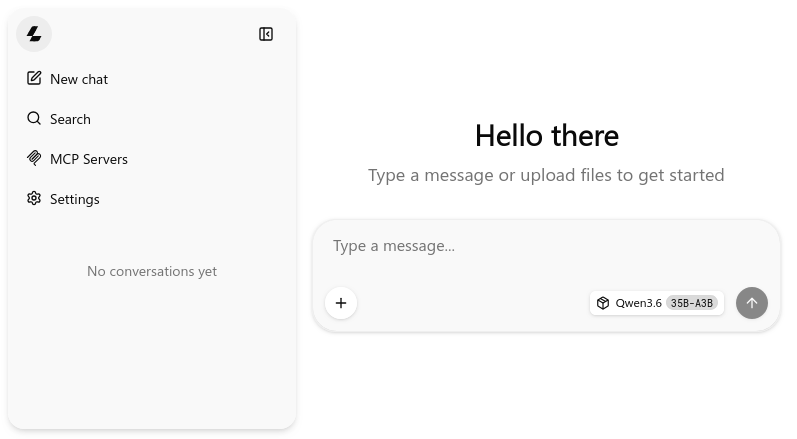
\includegraphics[width=0.8\textwidth]{assets/llama-ui.png}}
\caption{llama.cpp Web UI}
\label{fig:llama-ui}
\end{figure}

\subsection{Agentic Coding}

Now let's use \texttt{pi} with the local language model.

Pi is installed in the image \code{ghcr.io/codebar-shanghai/pi-docker-image:latest}. We will start it in another Docker container. Before we start the container, we need to prepare a configuration directory for Pi.

Create a folder for the Pi configuration. You can put it anywhere, and give it any name. In this example, I will use \texttt{c:\textbackslash{}pi-cfg} on Windows and \texttt{\textasciitilde{}/pi-cfg} on Linux / macOS.

Inside this folder, create another folder named \texttt{\textbf{agent}}. Then put the \texttt{\textbf{models.json}} inside the \texttt{agent} folder. The final structure should look like this:

\begin{minted}[formatcom=\treefont]{text}
~/pi-cfg
└── agent
    └── models.json
\end{minted}

Now start the Pi container:

\begin{minted}{bash}
docker run --rm -it \
  -v "$HOME/pi-cfg:/root/.pi" \
  ghcr.io/codebar-shanghai/pi-docker-image:latest \
  bash
\end{minted}

If you use Linux, use this command instead.

\begin{minted}{bash}
docker run --rm -it \
  --add-host=host.docker.internal:host-gateway \
  -v "$HOME/pi-cfg:/root/.pi" \
  ghcr.io/codebar-shanghai/pi-docker-image:latest \
  bash
\end{minted}

After the container starts, run these commands inside the container. You should see a welcome message like Figure~\ref{fig:starting-pi}.

\begin{minted}{bash}
# this is the working directory
mkdir helloworld-js

# now enter the working directory
cd helloworld-js

# now start pi
pi
\end{minted}

\begin{figure}[H]
\centering
\fbox{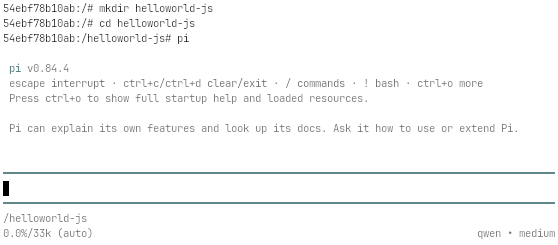
\includegraphics[]{assets/pi-welcome.png}}
\caption{Create a working directory and start Pi}
\label{fig:starting-pi}
\end{figure}

Now type this prompt and press Enter:

\begin{minted}{text}
Create a helloworld Node.js file
\end{minted}

You should see output similar to Figure~\ref{fig:pi-helloworld}.

\begin{figure}[H]
\centering
\fbox{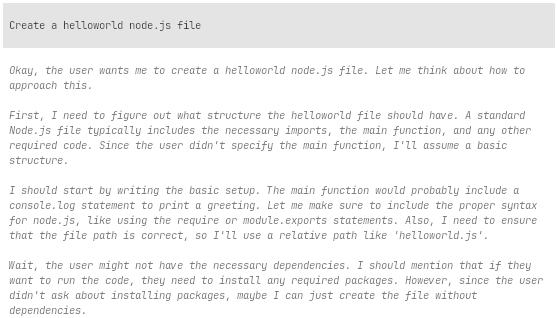
\includegraphics[]{assets/pi-helloworld.png}}
\caption{The output of Pi}
\label{fig:pi-helloworld}
\end{figure}

Now let's inspect the result. Type \verb|!ls| and press Enter to list the files in this working directory. In my case, Pi created a file named \texttt{main.js}.

Next type \verb|!cat main.js| to show the file content.

If the file looks good, type \verb|!node main.js| to run it.

The exclamation mark \texttt{!} tells Pi to run a shell command. After you press Enter, Pi changes the prompt to a dollar sign.

\begin{minted}{text}
$ ls
main.js

$ cat main.js

const fs = require('fs');

// This is a sample hello world
console.log('Hello, World!');

$ node main.js

Hello, World!
\end{minted}

If you know a little Node.js, you may notice that \texttt{const fs ...} is not needed in my result. This can happen because we are using a small model. Small models are easier to run, but they can make more mistakes. Your result may also look different from mine. We will talk more about models in the next chapter.

\subsection{Stop and Clean Up}

When you finish the workshop, you can stop the running tools.

In the Pi container, type \verb|/quit| and then type \verb|exit|.

For the llama.cpp server container, go back to the terminal where it is running. Press \texttt{Ctrl+C} to stop it.

If you don't need these images, you can delete them with these commands:

\begin{minted}{bash}
docker image rm ghcr.io/ggml-org/llama.cpp:server
docker image rm ghcr.io/codebar-shanghai/pi-docker-image:latest
\end{minted}

You can safely remove the downloaded \texttt{*.tar.gz} files, the model files, and \texttt{models.json}. If you do not need Docker anymore, you can uninstall it too.

\end{document}
